\newpage
\chapter{METODE PENELITIAN} \label{Bab III}

\section{Alur Penelitian} \label{sec:alur-penelitian}
Pada penelitian ini, alur dirancang untuk memastikan setiap tahapan pemrosesan dilakukan secara sistematis dan efisien. Alur penelitian ini mencerminkan langkah-langkah utama yang dilakukan pada penelitian ini, dapat dilihat pada Gambar \ref{fig:3.alur1} dan Gambar \ref{fig:3.alur2}. \par

\begin{figure}[H]
    \centering
    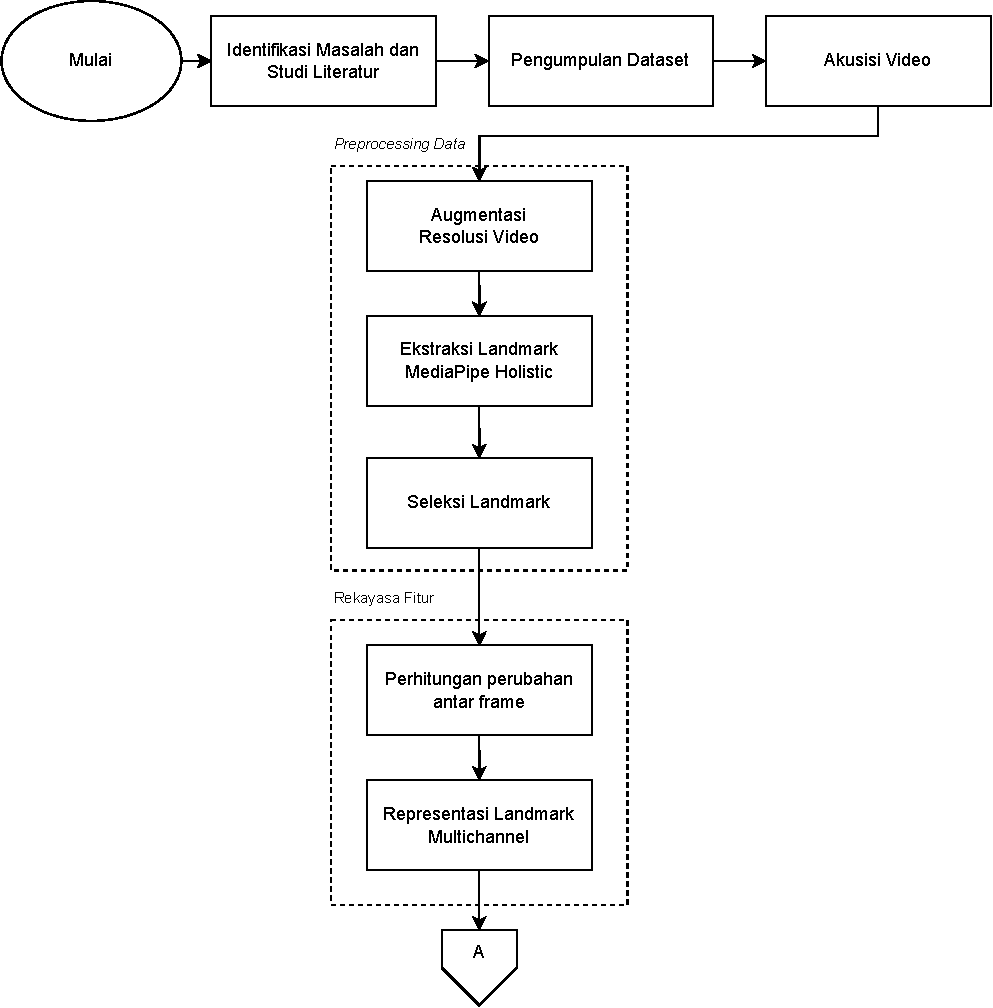
\includegraphics[width=1\textwidth]{figure/alur1.pdf}
    \caption{Tahap Identifikasi Masalah Hingga Rekayasa Fitur}
    \label{fig:3.alur1}
\end{figure} \par

\begin{figure}[H]
    \centering
    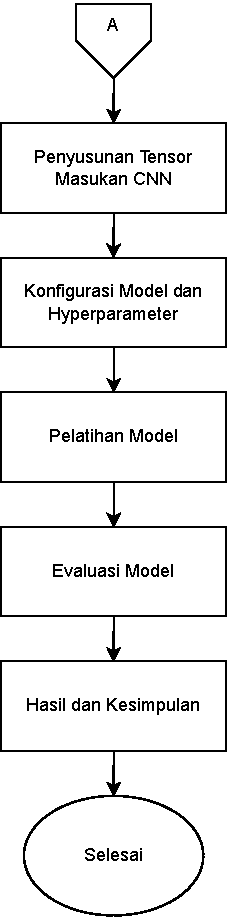
\includegraphics[width=0.23\textwidth]{figure/alur2.pdf}
    \caption{Tahap Penyusunan Tensor Hingga Hasil dan Kesimpulan}
    \label{fig:3.alur2}
\end{figure}

\section{Penjabaran Langkah Penelitian}
\label{sec:jabar-alur}

Penjelasan dari setiap langkah penelitian yang telah ditunjukkan pada bagian sebelumnya dijabarkan secara lebih komprehensif pada subbab berikut. 
Setiap tahapan dijelaskan secara sistematis untuk memberikan gambaran menyeluruh mengenai proses penelitian yang dilakukan. 
Uraian difokuskan pada alur metodologis tanpa membahas hasil eksperimen secara rinci. 
Pendekatan ini bertujuan untuk menjaga kejelasan antara tahapan metodologi dan analisis hasil penelitian.

\subsection{Identifikasi Masalah dan Studi Literatur}
\label{subsec:studi-identifikasi}

Tahapan awal penelitian diawali dengan identifikasi masalah yang berkaitan dengan pengenalan bahasa isyarat berbasis visual. 
Permasalahan utama yang diangkat adalah tingginya kompleksitas pendekatan berbasis pemodelan temporal eksplisit dalam pengenalan bahasa isyarat. 
Kondisi tersebut mendorong perlunya eksplorasi pendekatan alternatif yang lebih sederhana namun tetap efektif. 
Identifikasi masalah dilakukan dengan meninjau keterbatasan pendekatan yang umum digunakan pada penelitian terdahulu.

Studi literatur dilakukan untuk memperoleh pemahaman mendalam mengenai perkembangan penelitian \textit{Sign Language Recognition}. 
Literatur yang dikaji mencakup pendekatan berbasis model sekuensial, pemanfaatan \textit{landmark} tubuh manusia, serta penerapan CNN dua dimensi pada data berurutan. 
Kajian pustaka digunakan untuk mengidentifikasi celah penelitian yang belum banyak dieksplorasi. 
Hasil studi literatur menjadi dasar perumusan arah penelitian dan pemilihan metode yang digunakan.

% ------------------------------------------------
% CATATAN:
% - TIDAK perlu tabel atau gambar di subbab ini
% - Semua tabel literatur sudah ditempatkan di Bab II
% ------------------------------------------------


\subsection{Pengumpulan Dataset}
\label{subsec:pengumpulan-dataset}

Tahap pengumpulan dataset dilakukan untuk memperoleh data bahasa isyarat yang sesuai dengan kebutuhan penelitian. 
Dataset dikumpulkan dalam bentuk rekaman video bahasa isyarat dengan skema \textit{isolated sign}. 
Setiap isyarat direkam secara terpisah dengan batas awal dan akhir yang jelas. 
Pendekatan ini bertujuan untuk memudahkan proses segmentasi dan pelabelan data.

Pengumpulan dataset dilakukan secara terkontrol untuk menjaga konsistensi antar-sampel. 
Variasi gerakan tetap diperhatikan agar data mencerminkan perbedaan alami dalam melakukan isyarat. 
Dataset yang diperoleh kemudian digunakan sebagai dasar untuk proses akuisisi dan pengolahan data lebih lanjut. 
Tahap ini memastikan ketersediaan data yang representatif sebelum memasuki tahap pemrosesan teknis.

% ------------------------------------------------
% CATATAN:
% - TABEL BOLEH di sini (opsional):
%   Tabel ringkasan dataset (jumlah kelas, jumlah video, jumlah subjek)
% - TIDAK perlu gambar
% ------------------------------------------------


\subsection{Akuisisi Video Bahasa Isyarat}
\label{subsec:akusisi-data}

Akuisisi video bahasa isyarat dilakukan melalui proses perekaman langsung menggunakan perangkat kamera. 
Proses perekaman dilakukan dengan mempertimbangkan sudut pandang, pencahayaan, dan jarak kamera terhadap subjek. 
Pengaturan tersebut bertujuan untuk memastikan gerakan tangan dan tubuh terekam dengan jelas. 
Setiap video direkam dengan durasi yang cukup untuk merepresentasikan satu unit isyarat secara utuh.

Parameter teknis seperti resolusi video dan laju pengambilan frame disesuaikan agar mendukung proses ekstraksi \textit{landmark}. 
Konsistensi parameter perekaman dijaga pada seluruh sesi akuisisi data. 
Langkah ini bertujuan untuk meminimalkan variasi teknis yang dapat memengaruhi kualitas data. 
Video hasil akuisisi selanjutnya digunakan sebagai masukan pada tahap preprocessing.

% ------------------------------------------------
% CATATAN:
% - GAMBAR BOLEH:
%   Diagram setup kamera atau contoh frame hasil rekaman
% - TIDAK perlu tabel numerik detail
% ------------------------------------------------


\subsection{\textit{Preprocessing} Data}
\label{subsec:preprocessing-data}

Tahap preprocessing bertujuan untuk menyiapkan data video sebelum dilakukan rekayasa fitur dan pemodelan. 
Preprocessing difokuskan pada penyesuaian format data dan ekstraksi informasi visual awal. 
Tahapan ini memastikan data berada dalam kondisi yang konsisten dan siap diproses lebih lanjut. 
Proses preprocessing dilakukan secara berurutan untuk menjaga integritas data.

\subsubsection{Augmentasi Resolusi Video}
\label{subsubsec:augmentasi-resolusi}

Augmentasi resolusi video dilakukan untuk memperkaya variasi data tanpa menambah proses perekaman. 
Pada penelitian ini, seluruh video direkam menggunakan satu kamera dan satu subjek Tuli untuk menjaga konsistensi faktor biologis dan sudut pandang. 
Variasi resolusi diterapkan sebagai salah satu bentuk augmentasi yang mudah dikontrol dan direproduksi. 
Pendekatan ini mencerminkan perbedaan kualitas input yang dapat terjadi akibat penggunaan perangkat perekaman yang berbeda.

Video dengan resolusi awal selanjutnya diturunkan ke beberapa tingkat resolusi. 
Penurunan resolusi dilakukan tanpa mengubah rasio aspek video. 
Setiap versi resolusi diperlakukan sebagai sampel data yang terpisah. 
Langkah ini bertujuan untuk meningkatkan keragaman kualitas visual pada dataset.

Sebagai ilustrasi, Gambar \ref{fig:resolusi-asli} menunjukkan contoh frame video dengan resolusi awal hasil perekaman. 
Gambar \ref{fig:resolusi-menengah} dan Gambar \ref{fig:resolusi-rendah} menunjukkan contoh frame hasil augmentasi dengan resolusi yang lebih rendah. 
Perbedaan tingkat ketajaman visual pada setiap resolusi menggambarkan variasi kualitas citra yang mungkin ditemui pada perangkat perekaman yang berbeda. 
Ilustrasi ini digunakan untuk memperjelas kondisi data masukan sebelum tahap ekstraksi \textit{landmark}.

\subsubsection{Ekstraksi \textit{Landmark} MediaPipe Holistic}
\label{subsubsec:ekstraksi-landmark}

Ekstraksi \textit{landmark} dilakukan menggunakan MediaPipe Holistic untuk memperoleh representasi titik-titik kunci tubuh manusia pada setiap frame video. 
Setiap frame diproses secara independen tanpa mempertimbangkan informasi temporal antar-frame. 
Pendekatan ini menghasilkan keluaran berupa koordinat \textit{landmark} yang merepresentasikan posisi relatif bagian tubuh terhadap kamera. 
Seluruh proses ekstraksi dilakukan secara otomatis dan real-time.

MediaPipe Holistic menghasilkan beberapa kelompok \textit{landmark}, yaitu \textit{pose}, tangan kiri, tangan kanan, dan wajah. 
\textit{Landmark pose} merepresentasikan struktur tubuh bagian atas dan bawah, sedangkan \textit{landmark} tangan merepresentasikan struktur jari dan telapak tangan secara rinci. 
\textit{Landmark wajah} juga diekstraksi untuk mencatat informasi ekspresi non-manual. 
Tidak seluruh komponen \textit{landmark} yang dihasilkan digunakan pada tahap pemrosesan selanjutnya.

Setiap \textit{landmark} direpresentasikan dalam bentuk koordinat tiga dimensi \textit{(x, y, z)} yang telah dinormalisasi relatif terhadap dimensi frame. 
Koordinat \textit{x} dan \textit{y} merepresentasikan posisi pada bidang citra, sedangkan koordinat \textit{z} merepresentasikan kedalaman relatif terhadap kamera. 
Seluruh koordinat \textit{landmark} disimpan dalam format berkas \textit{JSON} untuk setiap urutan video. 
Format penyimpanan ini memudahkan proses pemanggilan ulang data pada tahap \textit{preprocessing} dan rekayasa fitur.

% ------------------------------------------------
% CATATAN:
% - GAMBAR WAJIB:
%   Frame video + overlay landmark MediaPipe
% - TIDAK perlu tabel
% ------------------------------------------------

\subsubsection{Seleksi \textit{Landmark}}
\label{subsubsec:seleksi-normalisasi}

Seleksi \textit{landmark} dilakukan untuk memfokuskan representasi data pada titik-titik yang relevan. 
Tidak seluruh \textit{landmark} hasil ekstraksi digunakan pada penelitian ini. 
Koordinat kedalaman tidak digunakan karena bersifat relatif dan kurang stabil. 
Proses seleksi bertujuan untuk mengurangi kompleksitas data tanpa menghilangkan informasi gerakan utama.

% ------------------------------------------------
% CATATAN:
% - TIDAK perlu tabel
% - TIDAK perlu gambar
% ------------------------------------------------

\subsection{Rekayasa Fitur (\textit{Feature Engineering})}
\subsubsection{Perhitungan Perubahan Antar-\textit{Frame}} \label{subsubsec:perhitungan-perubahan}
Perubahan posisi \textit{landmark} antar-frame dihitung untuk menangkap dinamika gerakan. 
Perhitungan dilakukan berdasarkan selisih koordinat dua frame berurutan. 
Pendekatan ini memungkinkan informasi temporal direpresentasikan secara implisit. 
Rumus perhitungan perubahan antar-frame mengikuti formulasi yang telah dijelaskan pada Bab II.

\subsubsection{Representasi \textit{Landmark Multichannel}} \label{subsubsec:representasi-multichannel}
Sebagai ilustrasi konseptual, Tabel \ref{tab:landmark-example} menunjukkan contoh representasi satu titik \textit{landmark} pada dua frame berurutan beserta perubahan posisinya. 
Nilai numerik pada tabel bersifat ilustratif dan tidak merepresentasikan data eksperimen sebenarnya. 
Ilustrasi ini bertujuan untuk memberikan gambaran konkret mengenai pembentukan fitur multichannel. 
Pendekatan ini membantu pembaca memahami konsep representasi tanpa bergantung pada dataset tertentu.

\begin{table}[H]
  \centering
  \caption{Ilustrasi representasi fitur \textit{landmark multichannel} untuk satu \textit{landmark} sepanjang waktu}
  \label{tab:landmark-multichannel-example}
  \begin{tabular}{|c|c|l|c|c|c|c|}
  \hline
  \textbf{Frame} & \textbf{Indeks} & \textbf{Nama \textit{Landmark}} & $x$ & $y$ & $dx$ & $dy$ \\ \hline
  $t-2$ & 0 & Wrist & 0.42 & 0.62 & --    & --    \\ \hline
  $t-1$ & 0 & Wrist & 0.45 & 0.60 & 0.03  & -0.02 \\ \hline
  $t$   & 0 & Wrist & 0.48 & 0.58 & 0.03  & -0.02 \\ \hline
  $t+1$ & 0 & Wrist & 0.50 & 0.56 & 0.02  & -0.02 \\ \hline
  $t+2$ & 0 & Wrist & 0.52 & 0.54 & 0.02  & -0.02 \\ \hline
  \end{tabular}

  \vspace{0.5em}
  {\footnotesize Catatan: Ilustrasi menunjukkan perubahan posisi satu \textit{landmark} (Wrist) pada beberapa frame berurutan.}
\end{table}  

Setiap \textit{landmark} direpresentasikan menggunakan empat kanal fitur, yaitu $(x, y, dx, dy)$. 
Seluruh \textit{landmark} pada setiap frame disusun secara berurutan membentuk representasi spasial multichannel. 
Representasi ini memungkinkan data gerakan diproses oleh CNN dua dimensi. 
Ilustrasi representasi \textit{landmark multichannel} ditunjukkan pada Tabel \ref{tab:landmark-multichannel-example}.


\subsection{Penyusunan Tensor Masukan CNN} \label{subsubsec:penyusunan-tensor}
Representasi \textit{landmark multichannel} selanjutnya disusun ke dalam bentuk tensor masukan CNN. 
Tensor masukan disusun mengikuti format kanal-terlebih-dahulu (\textit{channel-first}). 
Struktur tensor disesuaikan dengan arsitektur CNN dua dimensi yang digunakan. 
Penyusunan tensor ini menjadi penghubung antara tahap rekayasa fitur dan pemodelan.

\subsection{Konfigurasi Model dan \textit{Hyperparameter}} \label{subsec:konfigurasi-model-hyperparameter}
\subsubsection{Arsitektur ResNet-2D}
\subsubsection{Modifikasi Input \textit{Channel}}
\subsubsection{Konfigurasi \textit{Hyperparameter}}

\section{Alat dan Bahan} \label{sec:alat-bahan}
Dalam menjalani penelitian, beberapa alat dan bahan digunakan untuk memastikan penelitian berjalan dengan baik.\par
\subsection{Alat} \label{subsec:alat}
Dalam membuat pengukuran frekuensi denyut nadi non-kontak dalam penelitian, berikut adalah alat-alat yang digunakan: \par
\begin{enumerate}[noitemsep]
	\item \textit{Visual Studio Code} sebagai \textit{tools} untuk \textit{text editor}.
	\item Python versi 3.12.5
        \item OpenCV versi 4.10.0.84
	\item NumPy versi 2.1.1
	\item Mediapipe versi 0.10.14
	\item Scipy versi 1.12.0
        \item Matplotlib versi 3.8.3
        \item Flask versi 3.1.0
\end{enumerate}

\subsection{Bahan} \label{subsec:bahan}
Dataset yang digunakan pada penelitian ini merupakan dataset 

\section{Metode Evaluasi}
Evaluasi performa model dilakukan menggunakan metrik klasifikasi yang telah didefinisikan pada Bab II. 
Pengujian dilakukan pada data uji yang tidak digunakan selama proses pelatihan. 
Pendekatan ini bertujuan untuk menilai kemampuan generalisasi model. 
Hasil evaluasi dianalisis untuk menilai efektivitas pendekatan yang diusulkan.
\subsection{Metrik Evaluasi}
\subsection{Prosedur Pengujian}

\section{Ilustrasi Proses Pengolahan Data}
\subsection{Ilustrasi Input Video} \label{subsec:ilustrasi-input}
\subsection{Ilustrasi Ekstraksi \textit{Landmark}} \label{subsec:ilustrasi-ekstraksi}
\subsection{Ilustrasi Pembentukan Tensor} \label{subsec:ilustrasi-tensor}

